% This file: 			Prelim. draft for Heckman to see progress
% Contributors: 		Pietro Biroli, Daniela Del Boca, Linor Kiknadze, 
%					Yu Kyung Koh, Sylvi Kuperman, Sidharth Moktan, 
%					Chiara Pronzato, Nirali Trevedi, Anna Ziff
% Original date: 		10/10/16
% Project: 			Reggio Evaluation

%Style
\documentclass[12pt]{article}
\usepackage[top=1in, bottom=1in, left=1in, right=1in]{geometry}
\parindent 22pt
\usepackage{fancyhdr}

%Packages
\usepackage{adjustbox}
\usepackage{amsmath}
\usepackage{amsfonts}
\usepackage{amssymb}
\usepackage{bm}
\usepackage[table]{xcolor}
\usepackage{tabu}
\usepackage{makecell}
\usepackage{longtable}
\usepackage{multirow}
\usepackage[normalem]{ulem}
\usepackage{etoolbox}
\usepackage{graphicx}
\usepackage{tabularx}
\usepackage{ragged2e}
\usepackage{booktabs}
\usepackage{caption}
\usepackage{fixltx2e}
\usepackage[para, flushleft]{threeparttablex}
\usepackage[capposition=top]{floatrow}
\usepackage{subcaption}
\usepackage{pdfpages}
\usepackage{pdflscape}
\usepackage{natbib}
\usepackage{bibunits}
\definecolor{maroon}{HTML}{990012}
\usepackage[colorlinks=true,linkcolor=maroon,citecolor=maroon,urlcolor=maroon,anchorcolor=maroon]{hyperref}
\usepackage{marvosym}
\usepackage{makeidx}
\usepackage{tikz}
\usetikzlibrary{shapes}
\usepackage{setspace}
\usepackage{enumerate}
\usepackage{rotating}
\usepackage{epstopdf}
\usepackage[titletoc]{appendix}
\usepackage{framed}
\usepackage{comment}
\usepackage{xr}
\usepackage{titlesec}
\usepackage{footnote}
\usepackage{longtable}
\newlength{\tablewidth}
\setlength{\tablewidth}{9.3in}
\setcounter{secnumdepth}{4}

\titleformat{\paragraph}
{\normalfont\normalsize\bfseries}{\theparagraph}{1em}{}
\titlespacing*{\paragraph}
{0pt}{3.25ex plus 1ex minus .2ex}{1.5ex plus .2ex}
\makeatletter
\pretocmd\start@align
{%
  \let\everycr\CT@everycr
  \CT@start
}{}{}
\apptocmd{\endalign}{\CT@end}{}{}
\makeatother
%Watermark
\usepackage[printwatermark]{xwatermark}
\usepackage{lipsum}
\definecolor{lightgray}{RGB}{220,220,220}
%\newwatermark[allpages,color=lightgray,angle=45,scale=3,xpos=0,ypos=0]{Preliminary Draft}

%Further subsection level
\usepackage{titlesec}
\setcounter{secnumdepth}{4}
\titleformat{\paragraph}
{\normalfont\normalsize\bfseries}{\theparagraph}{1em}{}
\titlespacing*{\paragraph}
{0pt}{3.25ex plus 1ex minus .2ex}{1.5ex plus .2ex}

\setcounter{secnumdepth}{5}
\titleformat{\subparagraph}
{\normalfont\normalsize\bfseries}{\thesubparagraph}{1em}{}
\titlespacing*{\subparagraph}
{0pt}{3.25ex plus 1ex minus .2ex}{1.5ex plus .2ex}

%Functions
\DeclareMathOperator{\cov}{Cov}
\DeclareMathOperator{\var}{Var}
\DeclareMathOperator{\plim}{plim}
\DeclareMathOperator*{\argmin}{arg\,min}
\DeclareMathOperator*{\argmax}{arg\,max}

%Math Environments
\newtheorem{theorem}{Theorem}[section]
\newtheorem{claim}[theorem]{Claim}
\newtheorem{assumption}[theorem]{Assumption}
\newtheorem{definition}[theorem]{Definition}
\newtheorem{hypothesis}[theorem]{Hypothesis}
\newtheorem{property}[theorem]{Property}
\newtheorem{example}[theorem]{Example}
\newtheorem{condition}[theorem]{Condition}
\newtheorem{result}[theorem]{Result}
\newenvironment{proof}{\paragraph{Proof:}}{\hfill$\square$}

%Commands
\newcommand\independent{\protect\mathpalette{\protect\independenT}{\perp}}
\def\independenT#1#2{\mathrel{\rlap{$#1#2$}\mkern2mu{#1#2}}}
\newcommand{\overbar}[1]{\mkern 1.5mu\overline{\mkern-1.5mu#1\mkern-1.5mu}\mkern 1.5mu}
\newcommand{\equald}{\ensuremath{\overset{d}{=}}}
\captionsetup[table]{skip=10pt}
%\makeindex


\newcolumntype{L}[1]{>{\raggedright\let\newline\\\arraybackslash\hspace{0pt}}m{#1}}
\newcolumntype{C}[1]{>{\centering\let\newline\\\arraybackslash\hspace{0pt}}m{#1}}
\newcolumntype{R}[1]{>{\raggedleft\let\newline\\\arraybackslash\hspace{0pt}}m{#1}}



%Logo
%\AddToShipoutPictureBG{%
%  \AtPageUpperLeft{\raisebox{-\height}{\includegraphics[width=1.5cm]{uchicago.png}}}
%}

\newcolumntype{L}[1]{>{\raggedright\let\newline\\\arraybackslash\hspace{0pt}}m{#1}}
\newcolumntype{C}[1]{>{\centering\let\newline\\\arraybackslash\hspace{0pt}}m{#1}}
\newcolumntype{R}[1]{>{\raggedleft\let\newline\\\arraybackslash\hspace{0pt}}m{#1}} 

\newcommand{\mr}{\multirow}
\newcommand{\mc}{\multicolumn}

%\newcommand{\comment}[1]{}


\usepackage{sectsty}
\sectionfont{\fontsize{12}{12}\selectfont}
\subsectionfont{\fontsize{12}{12}\selectfont}

\begin{document}

\title{\normalsize \textbf{Evaluation of the Reggio Approach} \\ \normalsize Draft}
\author{\normalsize Reggio Team}
\date{\normalsize Original version: October 3, 2016 \\ Current version: \today}
\maketitle

\doublespacing

This draft presents (i) a brief description of the data, (ii) a simple analysis comparing individuals who attended the Reggio Emilia municipal schools to individuals in Reggio Emilia who did not attend any preschool, and (iii) a discussion of selection into preschool on observed characteristics. 

\section{Data}
\label{sec:data}

The sample is a subset of the individuals in Reggio Emilia, Parma, and Padova who were born in the year ranges of the five cohorts.  These individuals were collected from the population registries in each of the cities. The sample was then restricted to those individuals living in the same city in which they were raised. All cohorts except the youngest one were restricted to individuals who are Italian citizens. In contrast, the youngest cohort includes an oversampling of immigrant children. The sample from Reggio Emilia, across all cohorts, includes an oversampling of those who attended municipal schools, as this is considered the treatment.

Of the reference sample, 7,109 individuals were randomly selected. Of these, 4,019 completed interviews, resulting in a response rate of 56.5\%. Figure~\ref{fig:sample} presents an overview of the sample highlighting those who attended a Reggio Approach preschool. Table~\ref{tab:sample} provides a detailed tabulation of the sample by city, cohort, and school type.

\begin{figure}[H]
\begin{center}
\caption{The Sample by City and Cohort}\label{fig:sample}
	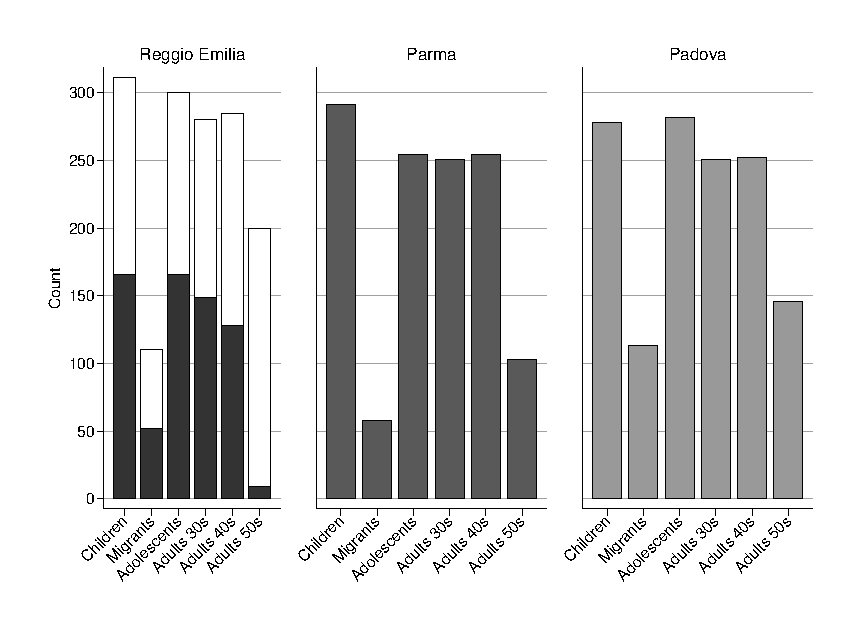
\includegraphics[width=.9\textwidth]{output/sample.eps}
\end{center}
\footnotetext{\noindent Note: This figure displays the number of individuals by cohort and city. The bars for Reggio Emilia differentiate between those who attended municipal preschool (black bars) and those who did not (white bars). Those in Reggio Emilia who attended municipal preschools are considered the treatment group.}
\end{figure}

\begin{table}[H]
\centering
\scalebox{0.7}{
\begin{threeparttable}
	\caption{The Sample by Cohort, City, and School Type}\label{tab:sample}
	\begin{tabular}{l*{15}{c}}
\toprule
            &\mc{5}{c}{Reggio Emilia: 1,471}   &     \mc{5}{c}{ Parma: 1,198}       &      \mc{5}{c}{Padova: 1,305}      \\
           \cmidrule(lr){2-6} \cmidrule(lr){7-11} \cmidrule(lr){12-16} 
      &        None&       Muni.&       State&      Relig.&       Priv.&        None&       Muni.&       State&      Relig.&       Priv.&        None&       Muni.&       State&      Relig.&       Priv.\\
\midrule
Children    &           2&         166&          45&          92&           5&           6&         154&          43&        77&           9&           2&          82&          40&         141&          12\\
Migrants    &           4&          52&          37&          14&           1&           4&          35&          10&          	3&           6&           5&          36&          47&          23&           1\\
Adolescents &           7&         166&          22&          96&           6&           4&         116&          43&     82&           6&           1&          93&          47&         131&           6\\
Adults 30    &          57&         149&          31&          40&           1&          44&          98&          51&        50&          5&       47&         35&         26&            140&    1 \\
Adults 40    &          80&         128&          17&          52&           5&         116&          52&          26&       55&          1&        75&      27 &            24&            123&  0 \\
Adults 50    &         147&           9&          10&          28&           2&          72&          12&           7&          11&           0 &        57&      11 &           2 &           68&    2 \\
\midrule
	       &         297&         670&         162&         322&          20&         246&         467&   180&    278&          27&      187&      284 &            186&        626& 22  \\
\bottomrule
\end{tabular}


\begin{tablenotes}
Note: This table shows the sample size by city, cohort, and school type. These numbers do not include individuals with an unidentified preschool type. In total, there are 45 individuals with unidentified preschool type. We separate migrants and children for clarity in this table even though they are in the same birth cohort (year of birth: 2006). None: no preschool; Muni.: municipal preschool;  State: state preschool; Relig.: religious preschool; Priv.: private preschool.
\end{tablenotes}
\end{threeparttable}
}
\end{table}

The structure of the cohorts allows us to study the effects of the Reggio Approach at different points throughout the life cycle. The youngest cohort of children were interviewed when they entered primary school, the adolescent cohort when they ended compulsory schooling, and the adult cohorts capture different points of adulthood to measure key outcomes such as engagement in the labor market, health, and family decisions. This cohort structure also allows us to evaluate the Reggio Approach compared to the alternative early childhood experiences as they evolved over time.

Separate questionnaires were administered to the children, adolescents, and adults, as well as to the caregivers of the children and adolescents. The questionnaires included items about early childhood experiences, family structure, education, interaction with non-Italians (or with Italians in the case of the migrant children), and measures of cognitive and social-emotional skills. The questionnaires for adults additionally included items about occupation, income, and life satisfaction. 

\section{Basic Analysis}
\label{sec:methodology}

We present a basic specification of OLS to estimate the effect of the Reggio Approach on an outcome of interest, $Y$, compared to not attending preschool at all. For this abbreviated analysis, we restrict to individuals from Reggio Emilia who either attended a Reggio Approach preschool or did not attend any preschool (across all cohorts, $N = 967$).

For individual $i$ in Reggio Emilia, let $\mu_i$ indicate whether that individual attended a Reggio Approach preschool. We select a vector, $\bm{X}_i$, of five baseline control variables with the lowest BIC to account for family background.\footnote{These variables are: \color{maroon}{forthcoming}} For each cohort, we estimate $\beta_1$ in the simple model

\begin{equation}
	Y_i = \beta_0 + \beta_1 \mu_i + \bm{X}_i\bm{\beta} + \varepsilon_i
	\label{eq:ra-v-none}
\end{equation}

\noindent where we $\varepsilon_i$ is a random disturbance. 

While this estimate is useful in gaining a basic understanding of the effect of the Reggio Approach, there is a clear selection issue. That is, the choice to enroll a child in the Reggio Approach and the choice to not enroll a child in any preschool are likely tied to family characteristics. After Section~\ref{sec:results} in which we present the estimates from Equation~\eqref{eq:ra-v-none}, we present a discussion of selection on observed characteristics.

\subsection{Results}
\label{sec:results}


We present the estimates of the methods described above for a handful of key outcomes.\footnote{We choose outcomes that are economically significant,  outcomes that have limited missing values, and outcomes with sufficient variation across individuals.}\footnote{A brief description on the outcomes is as follows: We rescale noncognitive outcomes, including SDQ score, Locus of Control, and Depression score, so that the higher value has a more socially positive meaning; \textbf{SDQ Composite - Child} is reported by mother, and \textbf{SDQ Composite} is self-reported; \textbf{IQ Score} is measured using Raven's Progressive Matrices; \textbf{How Much Child Likes School} is a single question with three answers, where 1 means ``A little", 2 means ``So so", and 3 means ``A lot";  \textbf{High School Grade} has the maximum scoring of 100; since the mean and variance is not always the same, we standardize the high school grade for each city, cohort, and high school type based on our data to have mean zero and unit variance; All the other measures reported in the estimation results are binary indicators.} Overall, very few outcomes show significant and consistent treatment effects of the Reggio Approach. The strongest results are shown when we compare the Reggio Approach with no preschool for the age-40 cohort. 

In the child cohort, as shown in Table \ref{ols-M-child-reg-pres}, the Reggio Approach increased positive SDQ scores when compared to children who attended other preschools (OLS). This result gets more positive after controlling for more background characteristics, or when comparing with children in Padova.\footnote{The estimated coefficient is still positive, but not statistically significant, when comparing with children in Parma (DiD).} Using PSM and AIPW to address issues of selection provides similar results as those of the OLS specification. The children are slightly more likely to be overweight and have worse health, although these estimates are not significant for all specifications. The other main outcomes do not show significant effects.

In the adolescent cohort, as shown in Table \ref{ols-M-adol-reg-pres}, adolescents who attended the Reggio Approach are significantly less likely to be depressed according to within Reggio Emilia analyses and DiD estimates with Parma and Padova. However, the propensity score matching with Parma and Padova adolescents do not show significant effect on depression. The Reggio Approach individuals are more likely to be obese than individuals who attended other types of preschool, and the estimate on obesity is consistent across most of the methods. Some methods show that Reggio Approach individuals are less likely to be involved in sport activities, which is consistent with the increase in obesity. 

In the adult cohorts, there are differences when we compare Reggio Approach individuals to other preschool group and to no preschool group. The comparison with no preschool group, shown in tables \ref{ols-M-adult30-reg-nopres} and \ref{ols-M-adult40-reg-nopres}, shows many more statistically significant estimates. In the comparison with the other preschool group, shown in tables \ref{ols-M-adult30-reg-pres} and \ref{ols-M-adult40-reg-pres}, the only outcomes that shows some significance across different methods is high school graduation and voting behavior in the age-40 cohort. OLS estimate shows that the Reggio Approach age-40 individuals are more likely to graduate from high school than other group. 

In the comparison with no preschool group, Reggio Approach individuals in age-40 group are more likely to be employed. Moreover, Reggio Approach people are significantly more likely to work more hours than other groups for both the age-30 and age-40 groups. OLS estimates show that the Reggio Approach people are significantly more likely to be obese when compared to no preschool group in Reggio Emilia, which aligns with the adolescent results. The age-40 Reggio Approach individuals have significant and positive effects on locus of control, depression score, and voting behaviors across many methodologies. 

% ========================================================================= %
% CHILD COHORT


\begin{table}[H] \caption{Estimation Results for Main Outcomes, Comparison to Non-RA Preschools, Child Cohort} \label{ols-M-child-reg-pres}
\scalebox{0.7}{\begin{tabular}{l c c c c c c c}
\toprule
 & NoneIt & BICIt & FullIt & DidPmIt & DidPvIt & AIPWnoneIt & AIPWpresIt \\
\midrule
SDQ Composite - Child &      0.64 & \textbf{      1.03 } & \textbf{      1.18 } &      0.80 &     -0.33 & \textbf{     2.27} & \textbf{     1.02} \\
& (     0.47) & (     0.46) & (     0.45) & (     0.71) & (     0.58) & (     2.46) & (     0.42) \\
Obese &      0.00 &      0.02 &      0.04 &      0.00 &      0.06 &      0.07 &      0.02 \\
& (     0.05) & (     0.05) & (     0.05) & (     0.06) & (     0.06) & (     0.19) & (     0.04) \\
Overweight & \textbf{      0.05 } &      0.04 &      0.05 & \textbf{      0.10 } &     -0.04 &      0.07 & \textbf{     0.05} \\
& (     0.03) & (     0.03) & (     0.04) & (     0.06) & (     0.04) & (     0.20) & (     0.04) \\
Health is Good &     -0.04 &     -0.03 &     -0.01 &     -0.11 &      0.00 & \textbf{     0.41} &     -0.00 \\
& (     0.05) & (     0.05) & (     0.05) & (     0.08) & (     0.05) & (     0.20) & (     0.03) \\
Not Excited to Learn &     -0.00 &      0.00 &     -0.00 &     -0.03 &      0.03 &     -0.08 &     -0.01 \\
& (     0.02) & (     0.02) & (     0.02) & (     0.03) & (     0.03) & (     0.19) & (     0.02) \\
Problems Sitting Still &      0.03 &      0.02 &      0.00 & \textbf{      0.10 } &      0.06 & \textbf{     0.14} &      0.01 \\
& (     0.03) & (     0.03) & (     0.03) & (     0.06) & (     0.04) & (     0.03) & (     0.03) \\
How Much Child Likes School &      0.01 &      0.03 &      0.03 &     -0.06 &     -0.07 & \textbf{     0.56} &      0.04 \\
& (     0.06) & (     0.06) & (     0.06) & (     0.08) & (     0.07) & (     0.32) & (     0.06) \\
\bottomrule
\end{tabular}
}
\vspace{1ex} \\
\footnotesize\raggedright{Note: This table shows the estimates of the coefficient for attending Reggio Approach preschools from multiple methods. We compare Reggio Approach individuals with those who attended other preschools. Column title indicates the corresponding control set and and model. \textbf{None} = OLS estimate with no control variables. \textbf{BIC} = OLS estimate with controls selected by Bayesian Information Criterion (BIC) and additional controls for male indicator, migrant indicator, and ITC attendance indicator. \textbf{Full} = OLS estimate with the full set of controls. \textbf{PSM} =  propensity score matching estimation. \textbf{AIPW} = augmented inverse propensity weighting estimation. \textbf{DidPm} = difference-in-difference estimate of (Reggio Muni - Parma Muni) - (Reggio Other - Parma Other). \textbf{PSMPm} = propensity score matching between Reggio Approach people and people who attended Parma preschools. \textbf{DidPv} = difference-in-difference estimate of (Reggio Muni - Padova Muni) - (Reggio Other - Padova Other). \textbf{PSMPv} = propensity score matching between Reggio Approach people and people who attended Padova preschools. Robust standard errors are reported in parentheses. Bold number shows that the estimate is statistically significant at the 15\% level. Number of observations used in estimation is reported in italic.}

\end{table}


\begin{table}[H] \caption{Estimation Results for Main Outcomes, Comparison to Non-RA Preschools, Adolescent Cohort} \label{ols-M-adol-reg-pres}
\scalebox{0.66}{\begin{tabular}{l c c c c c c}
\toprule
 & None & Bic & Full & DidPm & DidPv & AIPW \\
\midrule
SDQ Composite - Child &      0.00 &      0.02 &      0.35 &     -0.32 &      0.44 &      0.32 \\
& (     0.58 ) & (     0.57 ) & (     0.61 ) & (     0.76 ) & (     0.48 ) & (     0.55 ) \\
SDQ Composite &      0.71 &      0.52 &      0.56 &     -0.56 &     -0.09 &      0.20 \\
& (     0.62 ) & (     0.64 ) & (     0.70 ) & (     0.77 ) & (     0.64 ) & (     0.58 ) \\
Depression Score - positive & \textbf{      1.13 } &      1.16 & \textbf{      1.43 } & \textbf{     -1.40 } &     -0.54 & \textbf{     0.77} \\
& (     0.77 ) & (     0.83 ) & (     0.89 ) & (     0.82 ) & (     0.74 ) & (     0.80 ) \\
Obese & \textbf{      0.07 } & \textbf{      0.08 } & \textbf{      0.08 } &      0.07 &     -0.05 & \textbf{     0.08} \\
& (     0.04 ) & (     0.04 ) & (     0.04 ) & (     0.05 ) & (     0.05 ) & (     0.04 ) \\
Overweight &     -0.01 &     -0.01 &     -0.01 &      0.05 &     -0.02 &     -0.00 \\
& (     0.02 ) & (     0.02 ) & (     0.03 ) & (     0.04 ) & (     0.01 ) & (     0.02 ) \\
Health is Good &      0.05 & \textbf{      0.08 } &      0.08 &      0.00 &     -0.03 & \textbf{     0.08} \\
& (     0.06 ) & (     0.06 ) & (     0.06 ) & (     0.07 ) & (     0.06 ) & (     0.06 ) \\
Go To School & \textbf{      0.04 } & \textbf{      0.04 } & \textbf{      0.05 } & \textbf{      0.03 } &     -0.01 & \textbf{     0.05} \\
& (     0.02 ) & (     0.03 ) & (     0.03 ) & (     0.01 ) & (     0.02 ) & (     0.03 ) \\
How Much Child Likes School &     -0.13 & \textbf{     -0.18 } & \textbf{     -0.19 } & \textbf{     -0.23 } &     -0.08 &     -0.10 \\
& (     0.11 ) & (     0.12 ) & (     0.12 ) & (     0.15 ) & (     0.11 ) & (     0.12 ) \\
Trust Score &     -0.00 &     -0.10 &     -0.02 &     -0.31 &      0.07 &     -0.08 \\
& (     0.18 ) & (     0.18 ) & (     0.19 ) & (     0.23 ) & (     0.18 ) & (     0.16 ) \\
Days of Sport (Weekly) & \textbf{     -0.40 } &     -0.31 &     -0.29 &      0.35 &      0.20 &     -0.33 \\
& (     0.23 ) & (     0.24 ) & (     0.26 ) & (     0.28 ) & (     0.24 ) & (     0.24 ) \\
\bottomrule
\end{tabular}
}
\vspace{1ex} \\
\footnotesize\raggedright{Note: This table shows the estimates of the coefficient for attending Reggio Approach preschools from multiple methods. We compare Reggio Approach individuals with those who attended other preschools. Column title indicates the corresponding control set and and model. \textbf{None} = OLS estimate with no control variables. \textbf{BIC} = OLS estimate with controls selected by Bayesian Information Criterion (BIC) and additional controls for male indicator and ITC attendance indicator. \textbf{Full} = OLS estimate with the full set of controls. \textbf{PSM} =  propensity score matching estimation. \textbf{AIPW} = augmented inverse propensity weighting estimation. \textbf{DidPm} = difference-in-difference estimate of (Reggio Muni - Parma Muni) - (Reggio Other - Parma Other). \textbf{PSMPm} = propensity score matching between Reggio Approach people and people who attended Parma preschools. \textbf{DidPv} = difference-in-difference estimate of (Reggio Muni - Padova Muni) - (Reggio Other - Padova Other). \textbf{PSMPv} = propensity score matching between Reggio Approach people and people who attended Padova preschools. Robust standard errors are reported in parentheses. Bold number shows that the estimate is statistically significant at the 15\% level. Number of observations used in estimation is reported in italic.}
\end{table}




\begin{table}[H] \caption{Estimation Results for Main Outcomes, Comparison to Non-RA Preschools, Adult-30 Cohorts} \label{ols-M-adult30-reg-pres}
\scalebox{0.65}{\begin{tabular}{l c c c c c c}
\toprule
 & None & BIC & Full & AIPW & DidPm & DidPv \\
\midrule
IQ Score &     -0.04 &     -0.07 &     -0.05 &     -0.07 & \textbf{     -0.16 } &     -0.00 \\
& (     0.06 ) & (     0.05 ) & (     0.05 ) & (     0.06 ) & (     0.06 ) & (     0.08 ) \\
& \textit{ 153 } & \textit{ 153 } & \textit{ 153 } & \textit{ 153 } & \textit{ 299 } & \textit{ 326 } \\
IQ Factor &     -0.15 & \textbf{     -0.24 } &     -0.17 &     -0.22 & \textbf{     -0.50 } &     -0.08 \\
& (     0.16 ) & (     0.15 ) & (     0.15 ) & (     0.14 ) & (     0.18 ) & (     0.24 ) \\
& \textit{ 153 } & \textit{ 153 } & \textit{ 153 } & \textit{ 153 } & \textit{ 299 } & \textit{ 326 } \\
Graduate from High School &     -0.04 &     -0.03 &     -0.05 &     -0.06 & \textbf{      0.14 } & \textbf{     -0.11 } \\
& (     0.05 ) & (     0.05 ) & (     0.05 ) & (     0.04 ) & (     0.08 ) & (     0.07 ) \\
& \textit{ 153 } & \textit{ 153 } & \textit{ 153 } & \textit{ 153 } & \textit{ 299 } & \textit{ 326 } \\
High School Grade &      2.23 &      1.96 &      2.10 & \textbf{     2.26} &      2.57 &      2.28 \\
& (     1.55 ) & (     1.49 ) & (     1.58 ) & (     1.62 ) & (     3.34 ) & (     3.79 ) \\
& \textit{ 117 } & \textit{ 117 } & \textit{ 117 } & \textit{ 117 } & \textit{ 246 } & \textit{ 253 } \\
Max Edu: University &      0.04 &      0.04 &      0.03 &      0.02 & \textbf{      0.22 } & \textbf{      0.22 } \\
& (     0.07 ) & (     0.07 ) & (     0.07 ) & (     0.07 ) & (     0.10 ) & (     0.14 ) \\
& \textit{ 153 } & \textit{ 153 } & \textit{ 153 } & \textit{ 153 } & \textit{ 299 } & \textit{ 326 } \\
Employed &     -0.02 &     -0.02 &     -0.01 &     -0.02 &     -0.01 &     -0.04 \\
& (     0.03 ) & (     0.04 ) & (     0.04 ) & (     0.04 ) & (     0.07 ) & (     0.09 ) \\
& \textit{ 153 } & \textit{ 153 } & \textit{ 153 } & \textit{ 153 } & \textit{ 299 } & \textit{ 326 } \\
Hours Worked Per Week &      1.13 &      0.40 &      1.22 &      0.53 &      0.18 &      0.65 \\
& (     1.90 ) & (     2.04 ) & (     2.08 ) & (     2.22 ) & (     3.48 ) & (     3.97 ) \\
& \textit{ 123 } & \textit{ 123 } & \textit{ 123 } & \textit{ 123 } & \textit{ 266 } & \textit{ 292 } \\
Married or Cohabitating &      0.08 &      0.04 &      0.04 &      0.02 &      0.07 &      0.19 \\
& (     0.08 ) & (     0.08 ) & (     0.08 ) & (     0.09 ) & (     0.11 ) & (     0.14 ) \\
& \textit{ 153 } & \textit{ 153 } & \textit{ 153 } & \textit{ 153 } & \textit{ 299 } & \textit{ 326 } \\
Obese &     -0.02 &      0.04 &      0.00 &      0.02 &      0.09 &      0.05 \\
& (     0.07 ) & (     0.06 ) & (     0.06 ) & (     0.07 ) & (     0.09 ) & (     0.12 ) \\
& \textit{ 153 } & \textit{ 153 } & \textit{ 153 } & \textit{ 153 } & \textit{ 299 } & \textit{ 326 } \\
Overweight &      0.04 &     -0.01 &     -0.01 &     -0.01 &     -0.14 &      0.01 \\
& (     0.07 ) & (     0.06 ) & (     0.06 ) & (     0.06 ) & (     0.10 ) & (     0.11 ) \\
& \textit{ 153 } & \textit{ 153 } & \textit{ 153 } & \textit{ 153 } & \textit{ 299 } & \textit{ 326 } \\
Locus of Control - positive &      0.11 &      0.04 &      0.06 &      0.04 &     -0.11 &      0.24 \\
& (     0.12 ) & (     0.11 ) & (     0.12 ) & (     0.11 ) & (     0.22 ) & (     0.22 ) \\
& \textit{ 149 } & \textit{ 149 } & \textit{ 149 } & \textit{ 149 } & \textit{ 286 } & \textit{ 315 } \\
Depression Score - positive &      0.46 &     -0.53 &     -0.24 &     -0.63 &      0.17 &      0.45 \\
& (     1.05 ) & (     0.69 ) & (     0.67 ) & (     0.67 ) & (     1.25 ) & (     1.70 ) \\
& \textit{ 151 } & \textit{ 151 } & \textit{ 151 } & \textit{ 151 } & \textit{ 297 } & \textit{ 321 } \\
Ever Voted for Municipal &      0.02 &      0.00 &      0.01 &      0.01 &      0.06 & \textbf{      0.28 } \\
& (     0.08 ) & (     0.06 ) & (     0.07 ) & (     0.06 ) & (     0.08 ) & (     0.11 ) \\
& \textit{ 151 } & \textit{ 151 } & \textit{ 151 } & \textit{ 151 } & \textit{ 295 } & \textit{ 314 } \\
Ever Voted for Regional &     -0.01 &     -0.04 &     -0.03 &     -0.04 &      0.03 & \textbf{      0.34 } \\
& (     0.08 ) & (     0.07 ) & (     0.07 ) & (     0.07 ) & (     0.08 ) & (     0.11 ) \\
& \textit{ 151 } & \textit{ 151 } & \textit{ 151 } & \textit{ 151 } & \textit{ 295 } & \textit{ 314 } \\
\bottomrule
\end{tabular}
}
\vspace{1ex} \\
\footnotesize\raggedright{Note: This table shows the estimates of the coefficient for attending Reggio Approach preschools from multiple methods. We compare Reggio Approach individuals with those who attended other preschools. Column title indicates the corresponding control set and and model. \textbf{None} = OLS estimate with no control variables. \textbf{BIC} = OLS estimate with controls selected by Bayesian Information Criterion (BIC) and additional controls for male indicator and ITC attendance indicator. \textbf{Full} = OLS estimate with the full set of controls. \textbf{PSM} =  propensity score matching estimation. \textbf{AIPW} = augmented inverse propensity weighting estimation. \textbf{DidPm} = difference-in-difference estimate of (Reggio Muni - Parma Muni) - (Reggio Other - Parma Other). \textbf{PSMPm} = propensity score matching between Reggio Approach people and people who attended Parma preschools. \textbf{DidPv} = difference-in-difference estimate of (Reggio Muni - Padova Muni) - (Reggio Other - Padova Other). \textbf{PSMPv} = propensity score matching between Reggio Approach people and people who attended Padova preschools. Robust standard errors are reported in parentheses. Bold number shows that the estimate is statistically significant at the 15\% level. Number of observations used in estimation is reported in italic.}
\end{table}

\begin{table}[H] \caption{Estimation Results for Main Outcomes, Comparison to No Preschools, Age-30 Cohorts} \label{ols-M-adult30-reg-nopres}
\scalebox{0.65}{\begin{tabular}{l c c c c c c c c c}
\toprule
 & None & BIC & Full & PSM & AIPW & DidPm & PSMPm & DidPv & PSMPv \\
\midrule
IQ Factor & 0.14 & 0.03 & -0.05 & 0.15 & 0.05 & -0.24 & \textbf{-0.57} & -0.11 & \textbf{-0.28} \\
& (0.16) & (0.15) & (0.16) & (0.19) & (0.17) & (0.22) & (0.18) & (0.27) & (0.13) \\
& \textit{ 167 } & \textit{ 167 } & \textit{ 167 } & \textit{ 167 } & \textit{ 167 } & \textit{ 252 } & \textit{ 153 } & \textit{ 233 } & \textit{ 157 } \\
Graduate from High School & -0.03 & 0.02 & 0.03 & 0.03 & 0.03 & 0.12 & 0.00 & -0.05 & -0.01 \\
& (0.05) & (0.05) & (0.05) & (0.07) & (0.06) & (0.09) & (0.09) & (0.09) & (0.05) \\
& \textit{ 167 } & \textit{ 167 } & \textit{ 167 } & \textit{ 167 } & \textit{ 167 } & \textit{ 252 } & \textit{ 153 } & \textit{ 233 } & \textit{ 157 } \\
High School Grade & \textbf{ 4.54 } & \textbf{ 4.98 } & \textbf{ 4.62 } & \textbf{5.57} & \textbf{5.90} & 0.35 & \textbf{12.70} & 3.16 & \textbf{3.68} \\
& (2.01) & (2.13) & (2.26) & (1.98) & (2.49) & (4.46) & (2.56) & (4.19) & (2.19) \\
& \textit{ 123 } & \textit{ 123 } & \textit{ 123 } & \textit{ 123 } & \textit{ 123 } & \textit{ 194 } & \textit{ 118 } & \textit{ 176 } & \textit{ 118 } \\
High School Grade (Standardized) & \textbf{ 6.39 } & \textbf{ 6.88 } & \textbf{ 6.54 } & \textbf{6.91} & \textbf{7.63} & 4.50 & \textbf{4.87} & 6.16 & -0.79 \\
& (2.25) & (2.39) & (2.52) & (2.27) & (2.52) & (3.85) & (2.23) & (4.82) & (2.46) \\
& \textit{ 123 } & \textit{ 123 } & \textit{ 123 } & \textit{ 123 } & \textit{ 123 } & \textit{ 192 } & \textit{ 117 } & \textit{ 175 } & \textit{ 118 } \\
Max Edu: University & -0.07 & -0.03 & -0.04 & -0.02 & -0.01 & 0.01 & \textbf{-0.16} & -0.15 & 0.03 \\
& (0.07) & (0.07) & (0.07) & (0.08) & (0.07) & (0.12) & (0.08) & (0.15) & (0.07) \\
& \textit{ 167 } & \textit{ 167 } & \textit{ 167 } & \textit{ 167 } & \textit{ 167 } & \textit{ 252 } & \textit{ 153 } & \textit{ 233 } & \textit{ 157 } \\
Employed & 0.04 & 0.02 & 0.04 & 0.05 & 0.01 & \textbf{ 0.14 } & -0.02 & 0.03 & 0.08 \\
& (0.05) & (0.05) & (0.05) & (0.05) & (0.03) & (0.09) & (0.03) & (0.10) & (0.08) \\
& \textit{ 167 } & \textit{ 167 } & \textit{ 167 } & \textit{ 167 } & \textit{ 167 } & \textit{ 252 } & \textit{ 153 } & \textit{ 233 } & \textit{ 157 } \\
Hours Worked Per Week & \textbf{ 6.84 } & \textbf{ 4.30 } & \textbf{ 5.16 } & 2.80 & \textbf{3.57} & \textbf{ 9.35 } & 1.75 & 5.25 & 2.77 \\
& (2.73) & (2.76) & (2.80) & (2.94) & (2.69) & (4.39) & (3.52) & (4.97) & (3.14) \\
& \textit{ 140 } & \textit{ 140 } & \textit{ 140 } & \textit{ 140 } & \textit{ 140 } & \textit{ 223 } & \textit{ 134 } & \textit{ 206 } & \textit{ 138 } \\
Married or Cohabitating & -0.01 & -0.08 & -0.10 & -0.05 & -0.07 & -0.09 & 0.04 & -0.01 & -0.05 \\
& (0.08) & (0.08) & (0.08) & (0.09) & (0.09) & (0.13) & (0.11) & (0.16) & (0.10) \\
& \textit{ 167 } & \textit{ 167 } & \textit{ 167 } & \textit{ 167 } & \textit{ 167 } & \textit{ 252 } & \textit{ 153 } & \textit{ 233 } & \textit{ 157 } \\
Not Obese & -0.00 & -0.06 & -0.06 & -0.09 & -0.07 & 0.03 & \textbf{-0.24} & \textbf{ -0.25 } & 0.10 \\
& (0.07) & (0.06) & (0.06) & (0.07) & (0.07) & (0.11) & (0.05) & (0.14) & (0.09) \\
& \textit{ 167 } & \textit{ 167 } & \textit{ 167 } & \textit{ 167 } & \textit{ 167 } & \textit{ 252 } & \textit{ 153 } & \textit{ 233 } & \textit{ 157 } \\
Not Overweight & -0.07 & 0.01 & -0.02 & 0.03 & 0.01 & -0.00 & 0.15 & 0.00 & -0.07 \\
& (0.07) & (0.06) & (0.06) & (0.08) & (0.06) & (0.12) & (0.10) & (0.12) & (0.06) \\
& \textit{ 167 } & \textit{ 167 } & \textit{ 167 } & \textit{ 167 } & \textit{ 167 } & \textit{ 252 } & \textit{ 153 } & \textit{ 233 } & \textit{ 157 } \\
Locus of Control - positive & 0.07 & -0.05 & -0.08 & -0.11 & -0.03 & -0.15 & \textbf{0.63} & 0.04 & -0.02 \\
& (0.14) & (0.13) & (0.14) & (0.12) & (0.11) & (0.25) & (0.16) & (0.27) & (0.20) \\
& \textit{ 163 } & \textit{ 163 } & \textit{ 163 } & \textit{ 163 } & \textit{ 163 } & \textit{ 239 } & \textit{ 144 } & \textit{ 221 } & \textit{ 148 } \\
Depression Score - positive & 1.26 & -0.04 & -0.20 & 0.37 & 0.07 & 0.74 & -0.93 & -0.53 & -0.38 \\
& (0.97) & (0.85) & (0.91) & (0.97) & (0.95) & (1.57) & (1.59) & (1.90) & (1.00) \\
& \textit{ 165 } & \textit{ 165 } & \textit{ 165 } & \textit{ 165 } & \textit{ 165 } & \textit{ 250 } & \textit{ 152 } & \textit{ 230 } & \textit{ 156 } \\
Ever Voted for Municipal & 0.10 & 0.03 & 0.04 & -0.07 & 0.02 & -0.05 & \textbf{0.22} & -0.01 & \textbf{0.27} \\
& (0.08) & (0.06) & (0.06) & (0.09) & (0.05) & (0.09) & (0.09) & (0.13) & (0.09) \\
& \textit{ 164 } & \textit{ 164 } & \textit{ 164 } & \textit{ 164 } & \textit{ 164 } & \textit{ 248 } & \textit{ 152 } & \textit{ 223 } & \textit{ 152 } \\
Ever Voted for Regional & 0.05 & -0.02 & -0.01 & -0.09 & -0.02 & -0.05 & \textbf{0.23} & 0.06 & \textbf{0.22} \\
& (0.08) & (0.07) & (0.07) & (0.09) & (0.07) & (0.09) & (0.09) & (0.13) & (0.09) \\
& \textit{ 164 } & \textit{ 164 } & \textit{ 164 } & \textit{ 164 } & \textit{ 164 } & \textit{ 248 } & \textit{ 152 } & \textit{ 223 } & \textit{ 152 } \\
\bottomrule
\end{tabular}
}
\vspace{1ex} \\
\footnotesize\raggedright{Note: This table shows the estimates of the coefficient for attending Reggio Approach preschools from multiple methods. We compare Reggio Approach individuals with those who attended other preschools. Column title indicates the corresponding control set and and model. \textbf{None} = OLS estimate with no control variables. \textbf{BIC} = OLS estimate with controls selected by Bayesian Information Criterion (BIC) and additional controls for male indicator and ITC attendance indicator. \textbf{Full} = OLS estimate with the full set of controls. \textbf{PSM} =  propensity score matching estimation. \textbf{AIPW} = augmented inverse propensity weighting estimation. \textbf{DidPm} = difference-in-difference estimate of (Reggio Muni - Parma Muni) - (Reggio None - Parma None). \textbf{PSMPm} = propensity score matching between Reggio Approach people and Parma people who attended no preschool. \textbf{DidPv} = difference-in-difference estimate of (Reggio Muni - Padova Muni) - (Reggio None - Padova None). \textbf{PSMPv} = propensity score matching between Reggio Approach people and Padova people who attended no preschool. Robust standard errors are reported in parentheses. Bold number shows that the estimate is statistically significant at the 15\% level. Number of observations used in estimation is reported in italic.}
\end{table}





\begin{table}[H] \caption{Estimation Results for Main Outcomes, Comparison to Non-RA Preschools, Age-40 Cohorts} \label{ols-M-adult40-reg-pres}
\scalebox{0.65}{\begin{tabular}{l c c c c c c c}
\toprule
 & None & BIC & Full & PSM & AIPW & PSMPm & PSMPv \\
\midrule
IQ Factor & -0.15 & -0.12 & -0.14 & -0.11 & -0.18 & \textbf{-0.30} & \textbf{-0.25} \\
& (0.12) & (0.11) & (0.11) & (0.12) & (0.10) & (0.12) & (0.14) \\
& \textit{ 159 } & \textit{ 159 } & \textit{ 159 } & \textit{ 159 } & \textit{ 159 } & \textit{ 197 } & \textit{ 239 } \\
Graduate from High School & \textbf{ 0.13 } & \textbf{ 0.10 } & \textbf{ 0.12 } & 0.09 & 0.02 & 0.05 & 0.05 \\
& (0.07) & (0.07) & (0.07) & (0.07) & (0.06) & (0.05) & (0.04) \\
& \textit{ 159 } & \textit{ 159 } & \textit{ 159 } & \textit{ 159 } & \textit{ 159 } & \textit{ 197 } & \textit{ 239 } \\
High School Grade & -0.66 & -0.09 & 0.36 & -0.84 & 0.53 & \textbf{3.74} & \textbf{5.91} \\
& (1.56) & (1.65) & (1.71) & (1.64) & (1.78) & (1.81) & (1.67) \\
& \textit{ 117 } & \textit{ 117 } & \textit{ 117 } & \textit{ 117 } & \textit{ 117 } & \textit{ 161 } & \textit{ 188 } \\
High School Grade (Standardized) & -1.13 & -0.17 & 0.36 & 0.74 & 0.65 & -1.50 & 1.65 \\
& (2.07) & (2.22) & (2.28) & (2.40) & (2.74) & (1.77) & (1.96) \\
& \textit{ 116 } & \textit{ 116 } & \textit{ 116 } & \textit{ 116 } & \textit{ 116 } & \textit{ 159 } & \textit{ 188 } \\
Max Edu: University & 0.07 & 0.05 & 0.03 & 0.01 & 0.04 & \textbf{-0.15} & \textbf{-0.12} \\
& (0.06) & (0.05) & (0.05) & (0.07) & (0.06) & (0.07) & (0.06) \\
& \textit{ 159 } & \textit{ 159 } & \textit{ 159 } & \textit{ 159 } & \textit{ 159 } & \textit{ 197 } & \textit{ 239 } \\
Employed & 0.01 & 0.01 & 0.01 & 0.03 & 0.03 & -0.00 & \textbf{0.07} \\
& (0.03) & (0.04) & (0.04) & (0.04) & (0.04) & (0.03) & (0.03) \\
& \textit{ 159 } & \textit{ 159 } & \textit{ 159 } & \textit{ 159 } & \textit{ 159 } & \textit{ 197 } & \textit{ 239 } \\
Hours Worked Per Week & -0.90 & -1.17 & -1.28 & -1.71 & -0.08 & 0.22 & \textbf{5.21} \\
& (1.93) & (2.12) & (2.20) & (1.92) & (1.65) & (1.73) & (1.77) \\
& \textit{ 144 } & \textit{ 144 } & \textit{ 144 } & \textit{ 144 } & \textit{ 144 } & \textit{ 179 } & \textit{ 226 } \\
Married or Cohabitating & 0.03 & 0.02 & 0.02 & 0.01 & 0.01 & 0.10 & \textbf{0.11} \\
& (0.07) & (0.07) & (0.07) & (0.07) & (0.07) & (0.07) & (0.07) \\
& \textit{ 159 } & \textit{ 159 } & \textit{ 159 } & \textit{ 159 } & \textit{ 159 } & \textit{ 197 } & \textit{ 239 } \\
Not Obese & -0.04 & 0.02 & 0.04 & 0.03 & 0.06 & -0.07 & -0.08 \\
& (0.07) & (0.07) & (0.07) & (0.08) & (0.06) & (0.07) & (0.07) \\
& \textit{ 159 } & \textit{ 159 } & \textit{ 159 } & \textit{ 159 } & \textit{ 159 } & \textit{ 197 } & \textit{ 239 } \\
Not Overweight & 0.05 & 0.03 & 0.03 & -0.01 & -0.04 & 0.01 & -0.03 \\
& (0.07) & (0.07) & (0.07) & (0.07) & (0.07) & (0.07) & (0.06) \\
& \textit{ 159 } & \textit{ 159 } & \textit{ 159 } & \textit{ 159 } & \textit{ 159 } & \textit{ 197 } & \textit{ 239 } \\
Locus of Control - positive & 0.13 & 0.14 & 0.11 & 0.19 & 0.07 & 0.16 & -0.00 \\
& (0.14) & (0.14) & (0.14) & (0.17) & (0.15) & (0.14) & (0.13) \\
& \textit{ 156 } & \textit{ 156 } & \textit{ 156 } & \textit{ 156 } & \textit{ 156 } & \textit{ 192 } & \textit{ 231 } \\
Depression Score - positive & 0.56 & \textbf{ 1.37 } & 1.09 & 1.28 & 1.00 & -0.71 & -0.31 \\
& (0.92) & (0.84) & (0.89) & (0.90) & (0.86) & (0.85) & (0.84) \\
& \textit{ 156 } & \textit{ 156 } & \textit{ 156 } & \textit{ 156 } & \textit{ 156 } & \textit{ 197 } & \textit{ 237 } \\
Ever Voted for Municipal & -0.07 & 0.07 & 0.06 & 0.09 & \textbf{0.10} & \textbf{0.14} & 0.07 \\
& (0.08) & (0.07) & (0.07) & (0.06) & (0.06) & (0.07) & (0.07) \\
& \textit{ 151 } & \textit{ 151 } & \textit{ 151 } & \textit{ 151 } & \textit{ 151 } & \textit{ 191 } & \textit{ 218 } \\
Ever Voted for Regional & -0.05 & 0.08 & 0.07 & 0.10 & \textbf{0.10} & \textbf{0.27} & \textbf{0.14} \\
& (0.08) & (0.07) & (0.07) & (0.07) & (0.08) & (0.07) & (0.07) \\
& \textit{ 151 } & \textit{ 151 } & \textit{ 151 } & \textit{ 151 } & \textit{ 151 } & \textit{ 191 } & \textit{ 218 } \\
\bottomrule
\end{tabular}
}
\vspace{1ex} \\
\footnotesize\raggedright{Note: This table shows the estimates of the coefficient for attending Reggio Approach preschools from multiple methods. We compare Reggio Approach individuals with those who attended other preschools. Column title indicates the corresponding control set and and model. \textbf{None} = OLS estimate with no control variables. \textbf{BIC} = OLS estimate with controls selected by Bayesian Information Criterion (BIC) and additional controls for male indicator and ITC attendance indicator. \textbf{Full} = OLS estimate with the full set of controls. \textbf{PSM} =  propensity score matching estimation. \textbf{AIPW} = augmented inverse propensity weighting estimation. \textbf{PSMPm} = propensity score matching between Reggio Approach people and Parma people who attended no preschool.  \textbf{PSMPv} = propensity score matching between Reggio Approach people and Padova people who attended no preschool. Robust standard errors are reported in parentheses. DiD estimates is not available for this cohort due to unavailability of municipal preschool systems in Parma and Padova. Bold number shows that the estimate is statistically significant at the 15\% level. Number of observations used in estimation is reported in italic.}
\end{table}

\begin{table}[H] \caption{Estimation Results for Main Outcomes, Comparison to No Preschools, Age-40 Cohorts} \label{ols-M-adult40-reg-nopres}
\scalebox{0.65}{\begin{tabular}{l c c c c c c}
\toprule
 & None & BIC & Full & AIPW & DidPm & DidPv \\
\midrule
IQ Score &     -0.03 &     -0.02 &     -0.01 &     -0.02 &      0.04 &     -0.04 \\
& (     0.05 ) & (     0.05 ) & (     0.06 ) & (     0.05 ) & (     0.06 ) & (     0.05 ) \\
& \textit{ 170 } & \textit{ 170 } & \textit{ 170 } & \textit{ 170 } & \textit{ 382 } & \textit{ 375 } \\
IQ Factor &      0.01 &      0.01 &      0.04 &      0.00 &      0.18 &      0.09 \\
& (     0.13 ) & (     0.14 ) & (     0.16 ) & (     0.13 ) & (     0.16 ) & (     0.15 ) \\
& \textit{ 170 } & \textit{ 170 } & \textit{ 170 } & \textit{ 170 } & \textit{ 382 } & \textit{ 375 } \\
Graduate from High School &     -0.07 &     -0.01 &     -0.06 &     -0.01 &      0.03 &     -0.09 \\
& (     0.05 ) & (     0.05 ) & (     0.06 ) & (     0.06 ) & (     0.07 ) & (     0.07 ) \\
& \textit{ 170 } & \textit{ 170 } & \textit{ 170 } & \textit{ 170 } & \textit{ 382 } & \textit{ 375 } \\
High School Grade &      0.59 &      1.65 &      1.77 &      1.51 & \textbf{     -4.02 } &      2.46 \\
& (     1.51 ) & (     1.59 ) & (     1.86 ) & (     1.66 ) & (     2.50 ) & (     2.33 ) \\
& \textit{ 135 } & \textit{ 135 } & \textit{ 135 } & \textit{ 135 } & \textit{ 311 } & \textit{ 297 } \\
Max Edu: University &      0.01 &      0.06 & \textbf{      0.11 } &      0.06 &     -0.11 &     -0.06 \\
& (     0.06 ) & (     0.06 ) & (     0.06 ) & (     0.07 ) & (     0.08 ) & (     0.09 ) \\
& \textit{ 170 } & \textit{ 170 } & \textit{ 170 } & \textit{ 170 } & \textit{ 382 } & \textit{ 375 } \\
Employed & \textbf{      0.06 } & \textbf{      0.08 } &      0.05 & \textbf{     0.08} &      0.05 & \textbf{      0.09 } \\
& (     0.04 ) & (     0.03 ) & (     0.03 ) & (     0.04 ) & (     0.05 ) & (     0.06 ) \\
& \textit{ 169 } & \textit{ 169 } & \textit{ 169 } & \textit{ 169 } & \textit{ 381 } & \textit{ 374 } \\
Hours Worked Per Week & \textbf{      5.71 } & \textbf{      7.29 } & \textbf{      7.39 } & \textbf{     7.24} & \textbf{      4.92 } & \textbf{      7.19 } \\
& (     2.42 ) & (     2.39 ) & (     2.60 ) & (     2.95 ) & (     2.80 ) & (     3.07 ) \\
& \textit{ 151 } & \textit{ 151 } & \textit{ 151 } & \textit{ 151 } & \textit{ 358 } & \textit{ 355 } \\
Married or Cohabitating &      0.02 &      0.01 &      0.05 &      0.04 &     -0.10 &     -0.13 \\
& (     0.07 ) & (     0.07 ) & (     0.08 ) & (     0.07 ) & (     0.09 ) & (     0.10 ) \\
& \textit{ 170 } & \textit{ 170 } & \textit{ 170 } & \textit{ 170 } & \textit{ 382 } & \textit{ 375 } \\
Obese & \textbf{     -0.14 } &     -0.08 &     -0.01 &     -0.07 & \textbf{     -0.26 } &     -0.03 \\
& (     0.07 ) & (     0.08 ) & (     0.08 ) & (     0.07 ) & (     0.09 ) & (     0.10 ) \\
& \textit{ 170 } & \textit{ 170 } & \textit{ 170 } & \textit{ 170 } & \textit{ 382 } & \textit{ 375 } \\
Overweight &      0.03 &     -0.04 &     -0.07 &     -0.06 &     -0.01 &      0.04 \\
& (     0.07 ) & (     0.07 ) & (     0.07 ) & (     0.07 ) & (     0.09 ) & (     0.08 ) \\
& \textit{ 170 } & \textit{ 170 } & \textit{ 170 } & \textit{ 170 } & \textit{ 382 } & \textit{ 375 } \\
Locus of Control - positive &      0.14 & \textbf{      0.20 } & \textbf{      0.28 } & \textbf{     0.27} &      0.12 & \textbf{      0.31 } \\
& (     0.13 ) & (     0.13 ) & (     0.14 ) & (     0.14 ) & (     0.17 ) & (     0.17 ) \\
& \textit{ 165 } & \textit{ 165 } & \textit{ 165 } & \textit{ 165 } & \textit{ 364 } & \textit{ 357 } \\
Depression Score - positive & \textbf{      2.25 } & \textbf{      2.23 } & \textbf{      2.10 } & \textbf{     2.47} &      0.20 & \textbf{      2.26 } \\
& (     0.92 ) & (     0.95 ) & (     1.07 ) & (     0.99 ) & (     1.13 ) & (     1.18 ) \\
& \textit{ 168 } & \textit{ 168 } & \textit{ 168 } & \textit{ 168 } & \textit{ 380 } & \textit{ 371 } \\
Ever Voted for Municipal & \textbf{      0.19 } & \textbf{      0.12 } &      0.11 & \textbf{     0.14} &     -0.02 &     -0.09 \\
& (     0.08 ) & (     0.08 ) & (     0.08 ) & (     0.09 ) & (     0.10 ) & (     0.10 ) \\
& \textit{ 153 } & \textit{ 153 } & \textit{ 153 } & \textit{ 153 } & \textit{ 365 } & \textit{ 340 } \\
Ever Voted for Regional & \textbf{      0.20 } & \textbf{      0.14 } & \textbf{      0.13 } & \textbf{     0.16} &      0.05 &     -0.10 \\
& (     0.08 ) & (     0.08 ) & (     0.08 ) & (     0.08 ) & (     0.09 ) & (     0.10 ) \\
& \textit{ 153 } & \textit{ 153 } & \textit{ 153 } & \textit{ 153 } & \textit{ 365 } & \textit{ 340 } \\
\bottomrule
\end{tabular}
}
\vspace{1ex} \\
\footnotesize\raggedright{Note: This table shows the estimates of the coefficient for attending Reggio Approach preschools from multiple methods. We compare Reggio Approach individuals with those who attended other preschools. Column title indicates the corresponding control set and and model. \textbf{None} = OLS estimate with no control variables. \textbf{BIC} = OLS estimate with controls selected by Bayesian Information Criterion (BIC) and additional controls for male indicator and ITC attendance indicator. \textbf{Full} = OLS estimate with the full set of controls. \textbf{PSM} =  propensity score matching estimation. \textbf{AIPW} = augmented inverse propensity weighting estimation. \textbf{DidPm} = difference-in-difference estimate of (Reggio Muni - Parma Other) - (Reggio None - Parma None). \textbf{PSMPm} = propensity score matching between Reggio Approach people and Parma people who attended no preschool. \textbf{DidPv} = difference-in-difference estimate of (Reggio Muni - Padova Other) - (Reggio None - Padova None). \textbf{PSMPv} = propensity score matching between Reggio Approach people and Padova people who attended no preschool. Robust standard errors are reported in parentheses. Bold number shows that the estimate is statistically significant at the 15\% level. Number of observations used in estimation is reported in italic.}
\end{table}



\section{Discussion of Selection}
\label{sec:selection}

The selection into preschool, as well as the selection into a particular type of preschool, might be determined by social, demographic, and economic characteristics of the family. Some of these characteristics might be observed in our data, and other might be omitted. We begin our exploration of the selection on observed characteristics by presenting the distributions of parental education.

Figures~\ref{fig:momEdu} and~\ref{fig:dadEdu} present the distribution of parental educational attainment for individuals from each combination of city, cohort, and preschool type. Figure~\ref{fig:momEdu} shows that within Reggio Emilia, mothers of individuals who did not attend preschool have proportionally higher levels of high school and university education than mothers of individuals who attended some form of preschool. This difference is more pronounced for the older cohorts. Figure~\ref{fig:dadEdu} shows that a similar pattern persists when examining father's education. A clear pattern does not emerge when we compare parental educational attainment between individuals who attended different types of preschool in Reggio Emilia. This suggests that parental education might have played a larger role in the initial decision of sending an individual to preschool, as compared to the subsequent decision of choosing a particular type of preschool. Figures~\ref{fig:momEdu} and~\ref{fig:dadEdu} include analogous graphs for Parma and Padova.

Figure~\ref{fig:parentsEdu} examines the difference of educational attainment between mothers and fathers for individuals from each city-cohort combination. Each column represents the total proportion of individuals in each city-cohort combination whose fathers are more educated than mothers. Each column is further broken down into sections that calculate this proportion conditional on different levels of father's education. The figures show that total inequality in educational attainment is largest in Padova and smallest in Reggio Emilia, and that this ranking of total inequality is consistent across the three adult cohorts. Furthermore, for the older cohorts, the level of inequality is substantially larger in Padova compared to Reggio Emilia and Parma. Padova is similar to the other two cities by the time we reach the age 30 cohort. 


\begin{figure}[!htb]
	\begin{minipage}{1\textwidth}
	\centering
	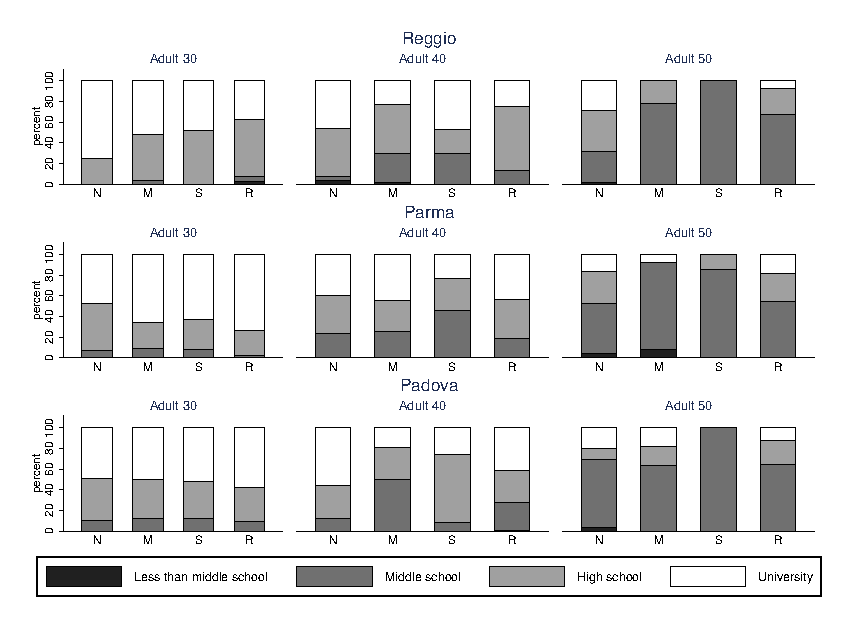
\includegraphics[scale=1.2]{../../Output/image/bar_momEdu}
	\caption{Mother's educational attainment by city, cohort and materna type}
	\label{fig:momEdu}
	\footnotetext{Note:  \textbf{(1)} Definiteion of bar labels: N = Not attended; M = Municipal; S = State; R = Religious. \textbf{(2)} Each bar presents the distribution of mothers' educational attainment for individuals in each city-cohort-materna type combination. }
	\end{minipage}
\end{figure}

\begin{figure}[!htb]
	\begin{minipage}{1\textwidth}
	\centering
	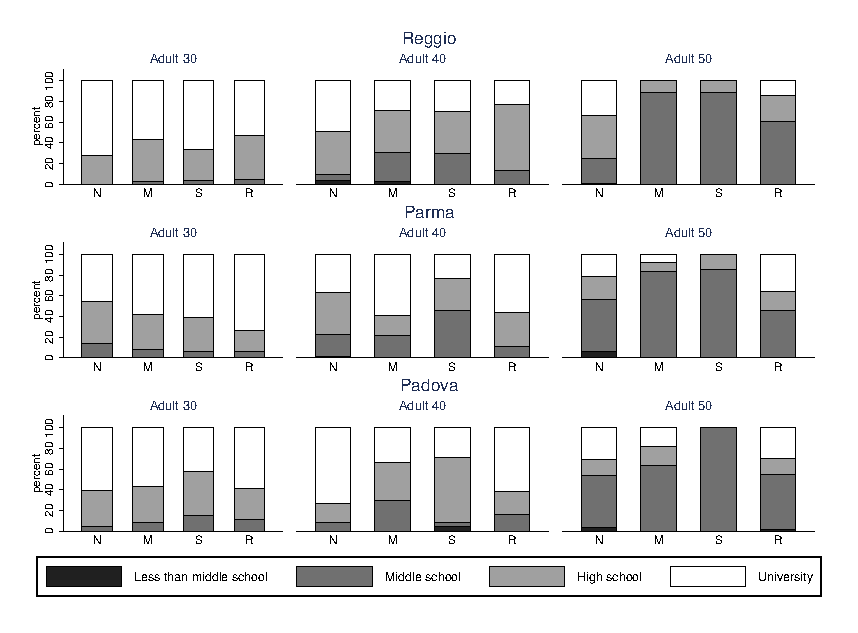
\includegraphics[scale=1.2]{../../Output/image/bar_dadEdu}
	\caption{Father's education attainment by city, cohort and materna type}
	\label{fig:dadEdu}
	\footnotetext{Note:  \textbf{(1)} Definition of bar labels: N = Not attended; M = Municipal; S = State; R = Religious. \textbf{(2)} Each bar presents the distribution of fathers' educational attainment for individuals in each city-cohort-materna type combination. }
	\end{minipage}
\end{figure}

\begin{figure}[!htb]
	\begin{minipage}{.9\textwidth}
	\centering
	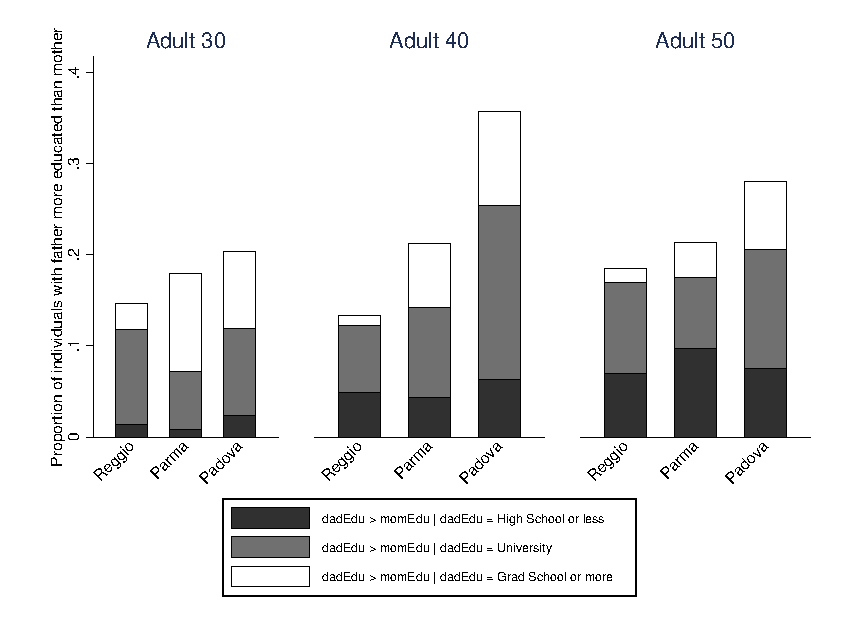
\includegraphics[scale=1]{../../Output/image/bar_parentsEduCompare}
	\caption{Proportion of individuals with fathers who are more educated than mothers by city and cohort}
	\label{fig:parentsEdu}
	\footnotetext{\noindent Note: Each column represents the proportion of individuals within each city-cohort combination whose fathers were more educated than their mothers.}
	\end{minipage}
\end{figure}

\clearpage

\bibliography{heckman}
\bibliographystyle{chicago}

\end{document}
